\documentclass{beamer}
\usetheme{Warsaw}
\usepackage[latin1]{inputenc}
\usepackage{tikz}
\usepackage{verbatim}
\usetikzlibrary{arrows,shapes}
\usetikzlibrary{matrix}

\begin{document}
\title{Regression Tree Training}   
\author{Frank Hutter}
\date{\today} 

\frame
{
\titlepage
} 

\begin{frame}

\frametitle{Regression Tree Training}

\begin{itemize}
\item In each internal node: only store split criterion used
\item In each leaf: store mean of runtimes
\end{itemize}

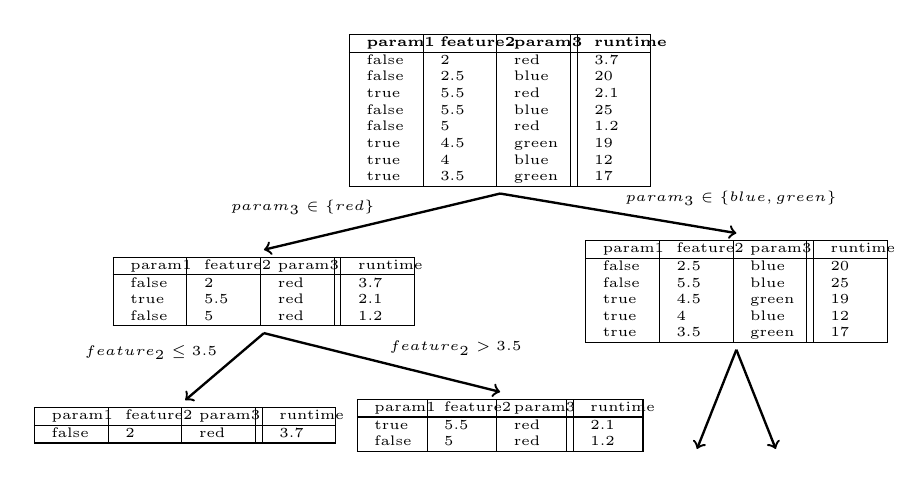
\begin{tikzpicture}
\fontsize{1.5}{6	}\selectfont

\uncover<2-> {
\node (A) at (4,0)
{\begin{tabular} { |p{0.5cm}|p{0.5cm}|p{0.5cm}||p{0.5cm}| } 

 \hline
 \textbf{param1} & \textbf{feature2} & \textbf{param3} & \textbf{runtime} \\ 
 \hline
 false & 2 & red & 3.7 \\
 false & 2.5 & blue & 20 \\
 true & 5.5 & red & 2.1 \\
 false & 5.5 & blue & 25 \\
 false & 5 & red & 1.2 \\
 true & 4.5 & green & 19 \\
 true & 4 & blue & 12 \\
 true & 3.5 & green & 17 \\ 
 \hline

\end{tabular}  } ;
}

\uncover<3-> {
\node (B) at (1,-2.3)
{\begin{tabular}{ |p{0.5cm}|p{0.5cm}|p{0.5cm}||p{0.5cm}| } 
 \hline
 param1 & feature2 & param3 & runtime \\ 
 \hline
 false & 2 & red & 3.7 \\
 true & 5.5 & red & 2.1 \\
 false & 5 & red & 1.2 \\
 \hline
\end{tabular}};
}

\uncover<3->{
\node (C) at (7,-2.3)
{\begin{tabular}{ |p{0.5cm}|p{0.5cm}|p{0.5cm}||p{0.5cm}| } 
 \hline
 param1 & feature2 & param3 & runtime \\ 
 \hline
 false & 2.5 & blue & 20 \\
 false & 5.5 & blue & 25 \\
 true & 4.5 & green & 19 \\
 true & 4 & blue & 12 \\
 true & 3.5 & green & 17 \\ 
 \hline
\end{tabular}};
}


\uncover<4->{	
\node (D) at (0,-4)
{\begin{tabular}{ |p{0.5cm}|p{0.5cm}|p{0.5cm}||p{0.5cm}| } 
 \hline
 param1 & feature2 & param3 & runtime \\ 
 \hline
 false & 2 & red & 3.7 \\
 \hline
\end{tabular}};
}

\uncover<4->{
\node (E) at (4,-4)
{\begin{tabular}{ |p{0.45cm}|p{0.45cm}|p{0.45cm}||p{0.45cm}| } 
 \hline
 param1 & feature2 & param3 & runtime \\ 
 \hline
  true & 5.5 & red & 2.1 \\
 false & 5 & red & 1.2 \\
 \hline
\end{tabular}};
}

\uncover<3-> {
\draw[line width=0.3mm, ->] (A.south)  --   node[above left=0cm] {$ param_3 \in \{red\} $} (B.north);
}
\uncover<3-> {
\draw[line width=0.3mm, ->] (A.south) -- node[auto] {$ param_3 \in \{blue, green\} $} (C.north);
}
\uncover<4-> {
\draw[line width=0.3mm, ->] (B.south) -- node[above left=0cm] {$feature_2 \leq 3.5$} (D.north);
}
\uncover<4-> {
\draw[line width=0.3mm, ->] (B.south) -- node[auto] {$feature_2 > 3.5$} (E.north);
}
\uncover<5-> {
\draw[line width=0.3mm, ->] (C.south) -- node[auto]  {} (7.5,-4.3);
}
\uncover<5-> {
\draw[->, line width=0.3mm] (C.south)  -- node[above] {}  (6.5,-4.3);
}
\end{tikzpicture}

\end{frame}



\frame
{
\frametitle{Regression Tree Predictions} 


}

\begin{frame}
\frametitle{Regression Tree Predictions}
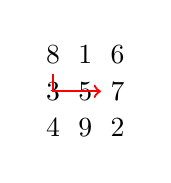
\begin{tikzpicture}
\matrix (magic) [matrix of nodes,ampersand replacement=\&]
{
8 \& 1 \& 6 \\
3 \& 5 \& 7 \\
4 \& 9 \& 2 \\
};
\draw[thick,red,->] (magic-1-1) |- (magic-2-3);
\end{tikzpicture}

\end{frame}



\end{document}
